\chapter{Logistic Regression of the HMM Hidden State Distribution} \label{chap:logreg_hmm} 

\section{Background}
A powerful way to use predictive models is to combine them. One possible way to do so is to use a hidden markov model to infer the hidden state of an entity each time slice, and then use the probability distribution outcomes of the hidden state as features for another predictive model. Applying HMM inference gives the probabilities at being in each hidden state for a given time-slice. These probabilities are used as features for the next classifier. In this example, we use the hidden state probability distribution as features for a time-slice, and apply logistic regression with the resulting feature-vector. We call this model logistic regression on HMM state.

For example, let's say that we want to apply logistic regression on the HMM hidden state distribution for a hidden state support of 3, lag of 3 and lead of 5. To perform inference on the HMM model, we would pass 3 weeks of data to the model, and ask for the hidden state probability distribution for each of three weeks. Each week would have a 3 element distribution (because there are 3 hidden states). Figure \ref{fig:hmm_as_logreg} shows a diagram of how the logistic regression feature vector is created. Only two of these are relevant (because the 3 numbers always add to 1). Next, we would take the first two probabilities from each of the 3 week's distributions, and use these 6 probabilities as a feature vector in logistic regression. The label of the data point is the stopout value for week 8.

\begin{figure}[!ht]
  \caption{Diagram showing how the logistic regression feature vector is created using the HMM hidden state probabilities as features.}\label{fig:hmm_as_logreg}
  \centering
    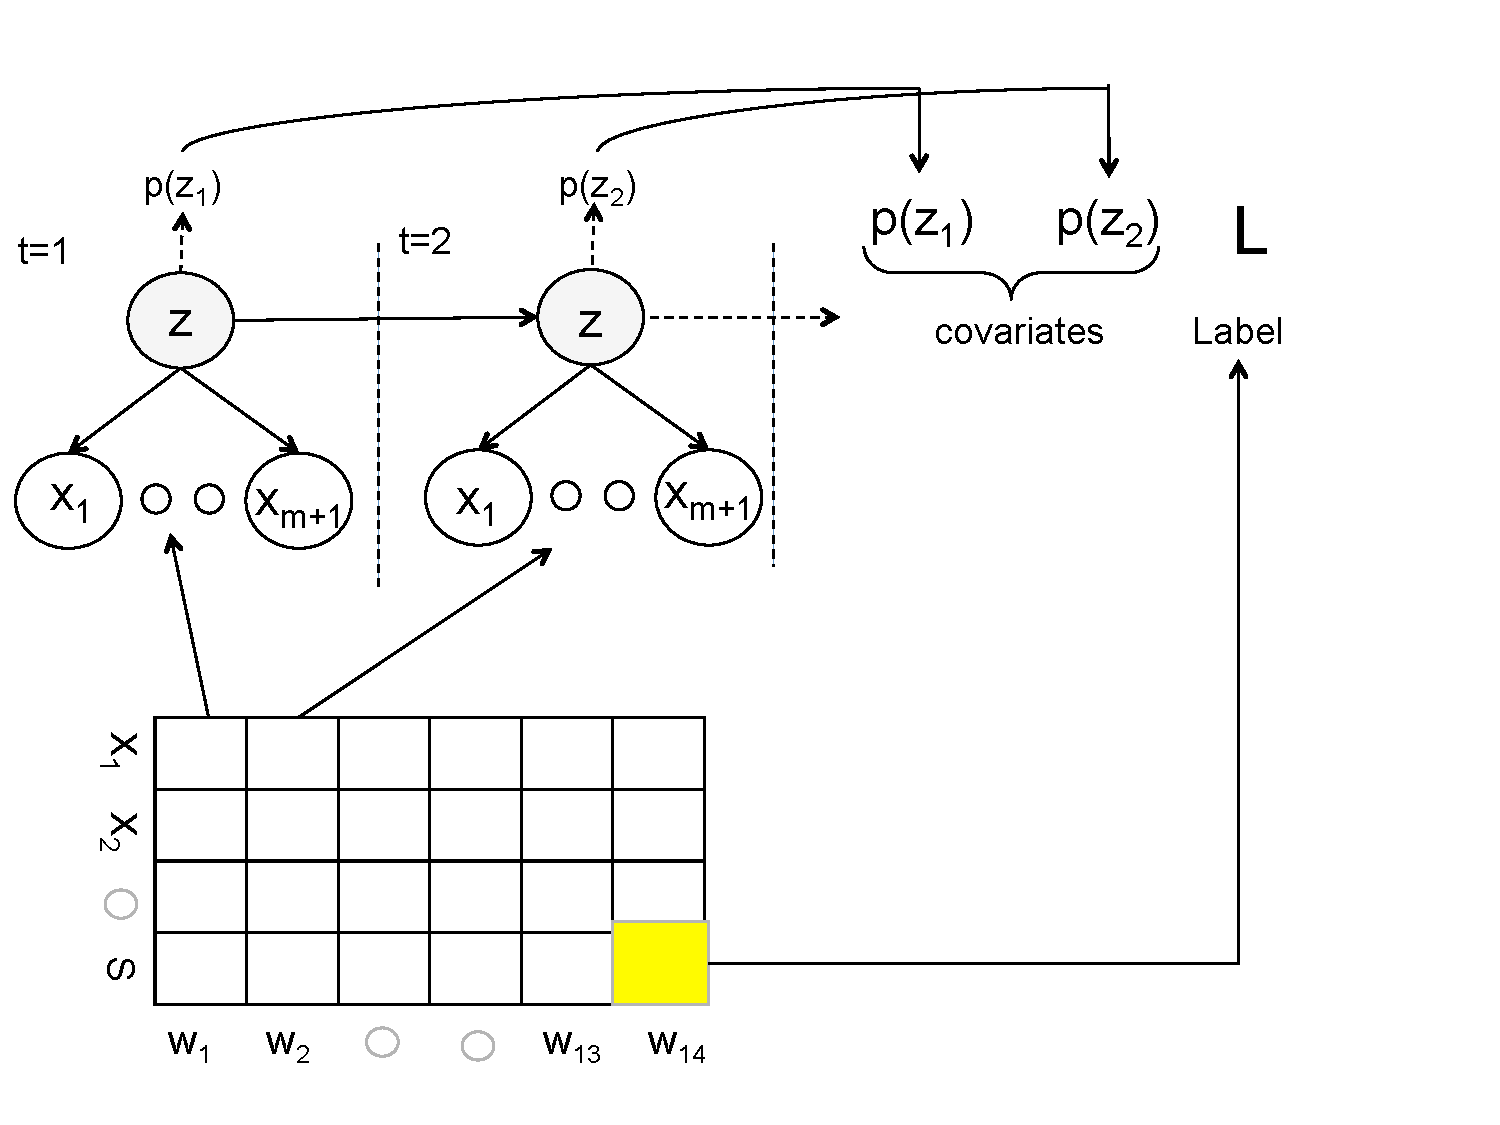
\includegraphics[width=0.8\textwidth]{figures/hmm_as_logreg}
\end{figure}

The intuition for why this might be a valid approach is that, in a way, the hidden state is a less noisy description of the observed variables. For example, in the stopout problem, the hidden state could represent the type of student, and the features are simply noisy observations. Constructing an HMM thus creates a less noisy description of the data. 

\section{Predicting stopout using logistic regression on HMM state}
We used the same parameters and software as in the individual models. This included a range of supports from 3 to 29, with a step size of 2, a maximum number of Baum-Welch iterations of 100, and a log-likelihood differential threshold of 0.0000001.

\subsection{Experimental setup}
The process to construct such a model is more complex than the previous two models. It entails the following, for each lead, lag and hidden support combination:
\begin{enumerate}
\item Split the train dataset into two equal partitions. I call the first `construct hmm' and the second `generate features'. We partition the data in order to not pollute the inference of the HMM with data it has been trained on.
\item Train an HMM on the `construct hmm' partition. Similarly to the normal HMM case, we trained 10 models to compensate for the potential to get stuck on a local maximum. We selected the best model to use based on the likelihood score of the Baum-Welch algorithm. We also performed this in parallel, as training can take significant amounts of time. We train this HMM once for each support, but use the same model for each lead and lag combination
\item Perform inference on the `generate features' partition. We asked the model to generate the hidden state probability distribution for each week in lag weeks, and took K -1 of these probabilities for each lag week as features for the model (where K is the hidden support). These feature vectors and labels become the training dataset for logistic regression.
\item Perform 10 fold cross validation, using the generated training dataset. 
\item Train a logistic regression model on the generated training dataset.
\item Perform inference on the actual test dataset by putting each data point through the model and comparing the resulting probability of stopout versus the truth stopout label.
\item Evaluate the model using mean cross-validation ROC AUC and test set ROC AUC.
\end{enumerate}

\section{Logistic regression on HMM state results}
Figures \ref{fig:hmm_logreg_heatmap_no_collab} through \ref{fig:hmm_logreg_heatmap_wiki_only} summarize the AUC of the receiver operating characteristic for all four cohorts over each lead and \lag combinations, similar to those in Chapter \ref{chap:logreg}. In order to compare, we choose the K with the best mean AUC for all 91 experiments. The chosen mean is indicated.

\begin{figure}[ht!]
  \caption{Heatmap of the \neither cohort. PCA transformations of features used. The shown heatmap used a support of 27 for the HMM. This was the support which yielded the highest mean AUC.}\label{fig:hmm_logreg_heatmap_no_collab}
  \centering
    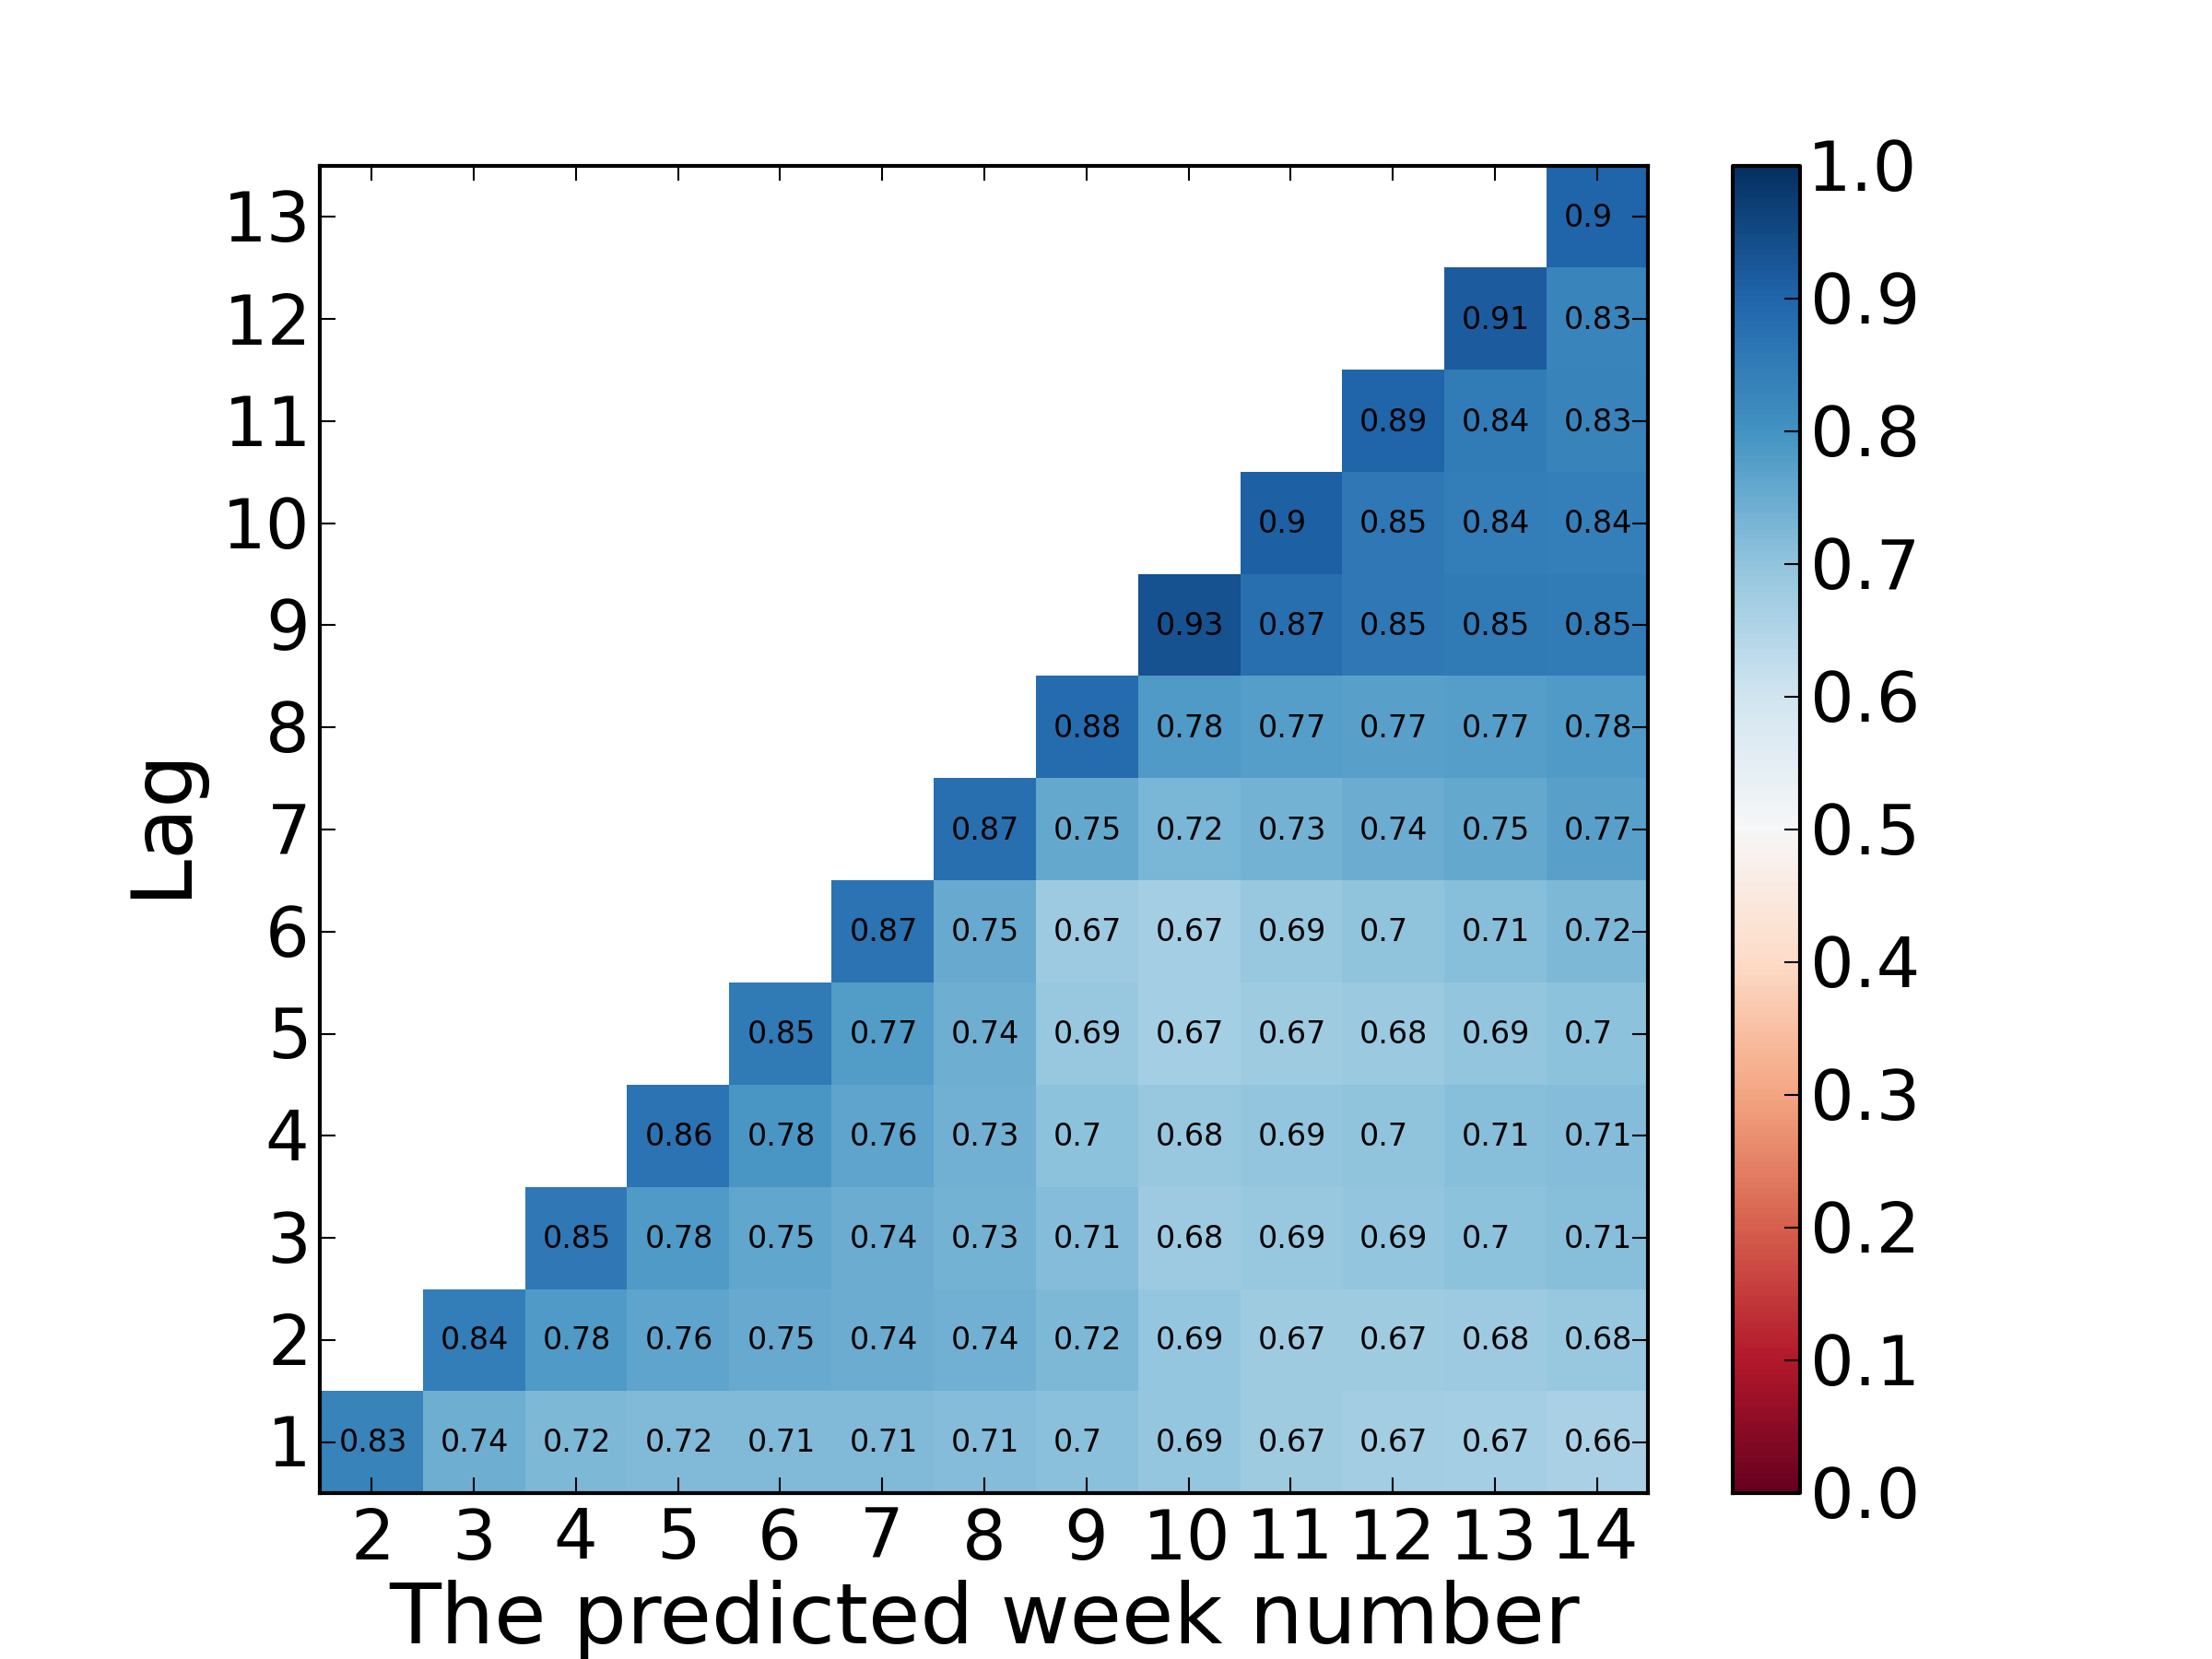
\includegraphics[width=1.0\textwidth]{figures/hmm_logreg/no_collab_pca_support_27.png}
\end{figure}

\begin{figure}[ht!]
  \caption{Heatmap of the \forum cohort. PCA transformations of features used. The shown heatmap used a support of 21 for the HMM. This was the support which yielded the highest mean AUC.}\label{fig:hmm_logreg_heatmap_forum_only}
  \centering
    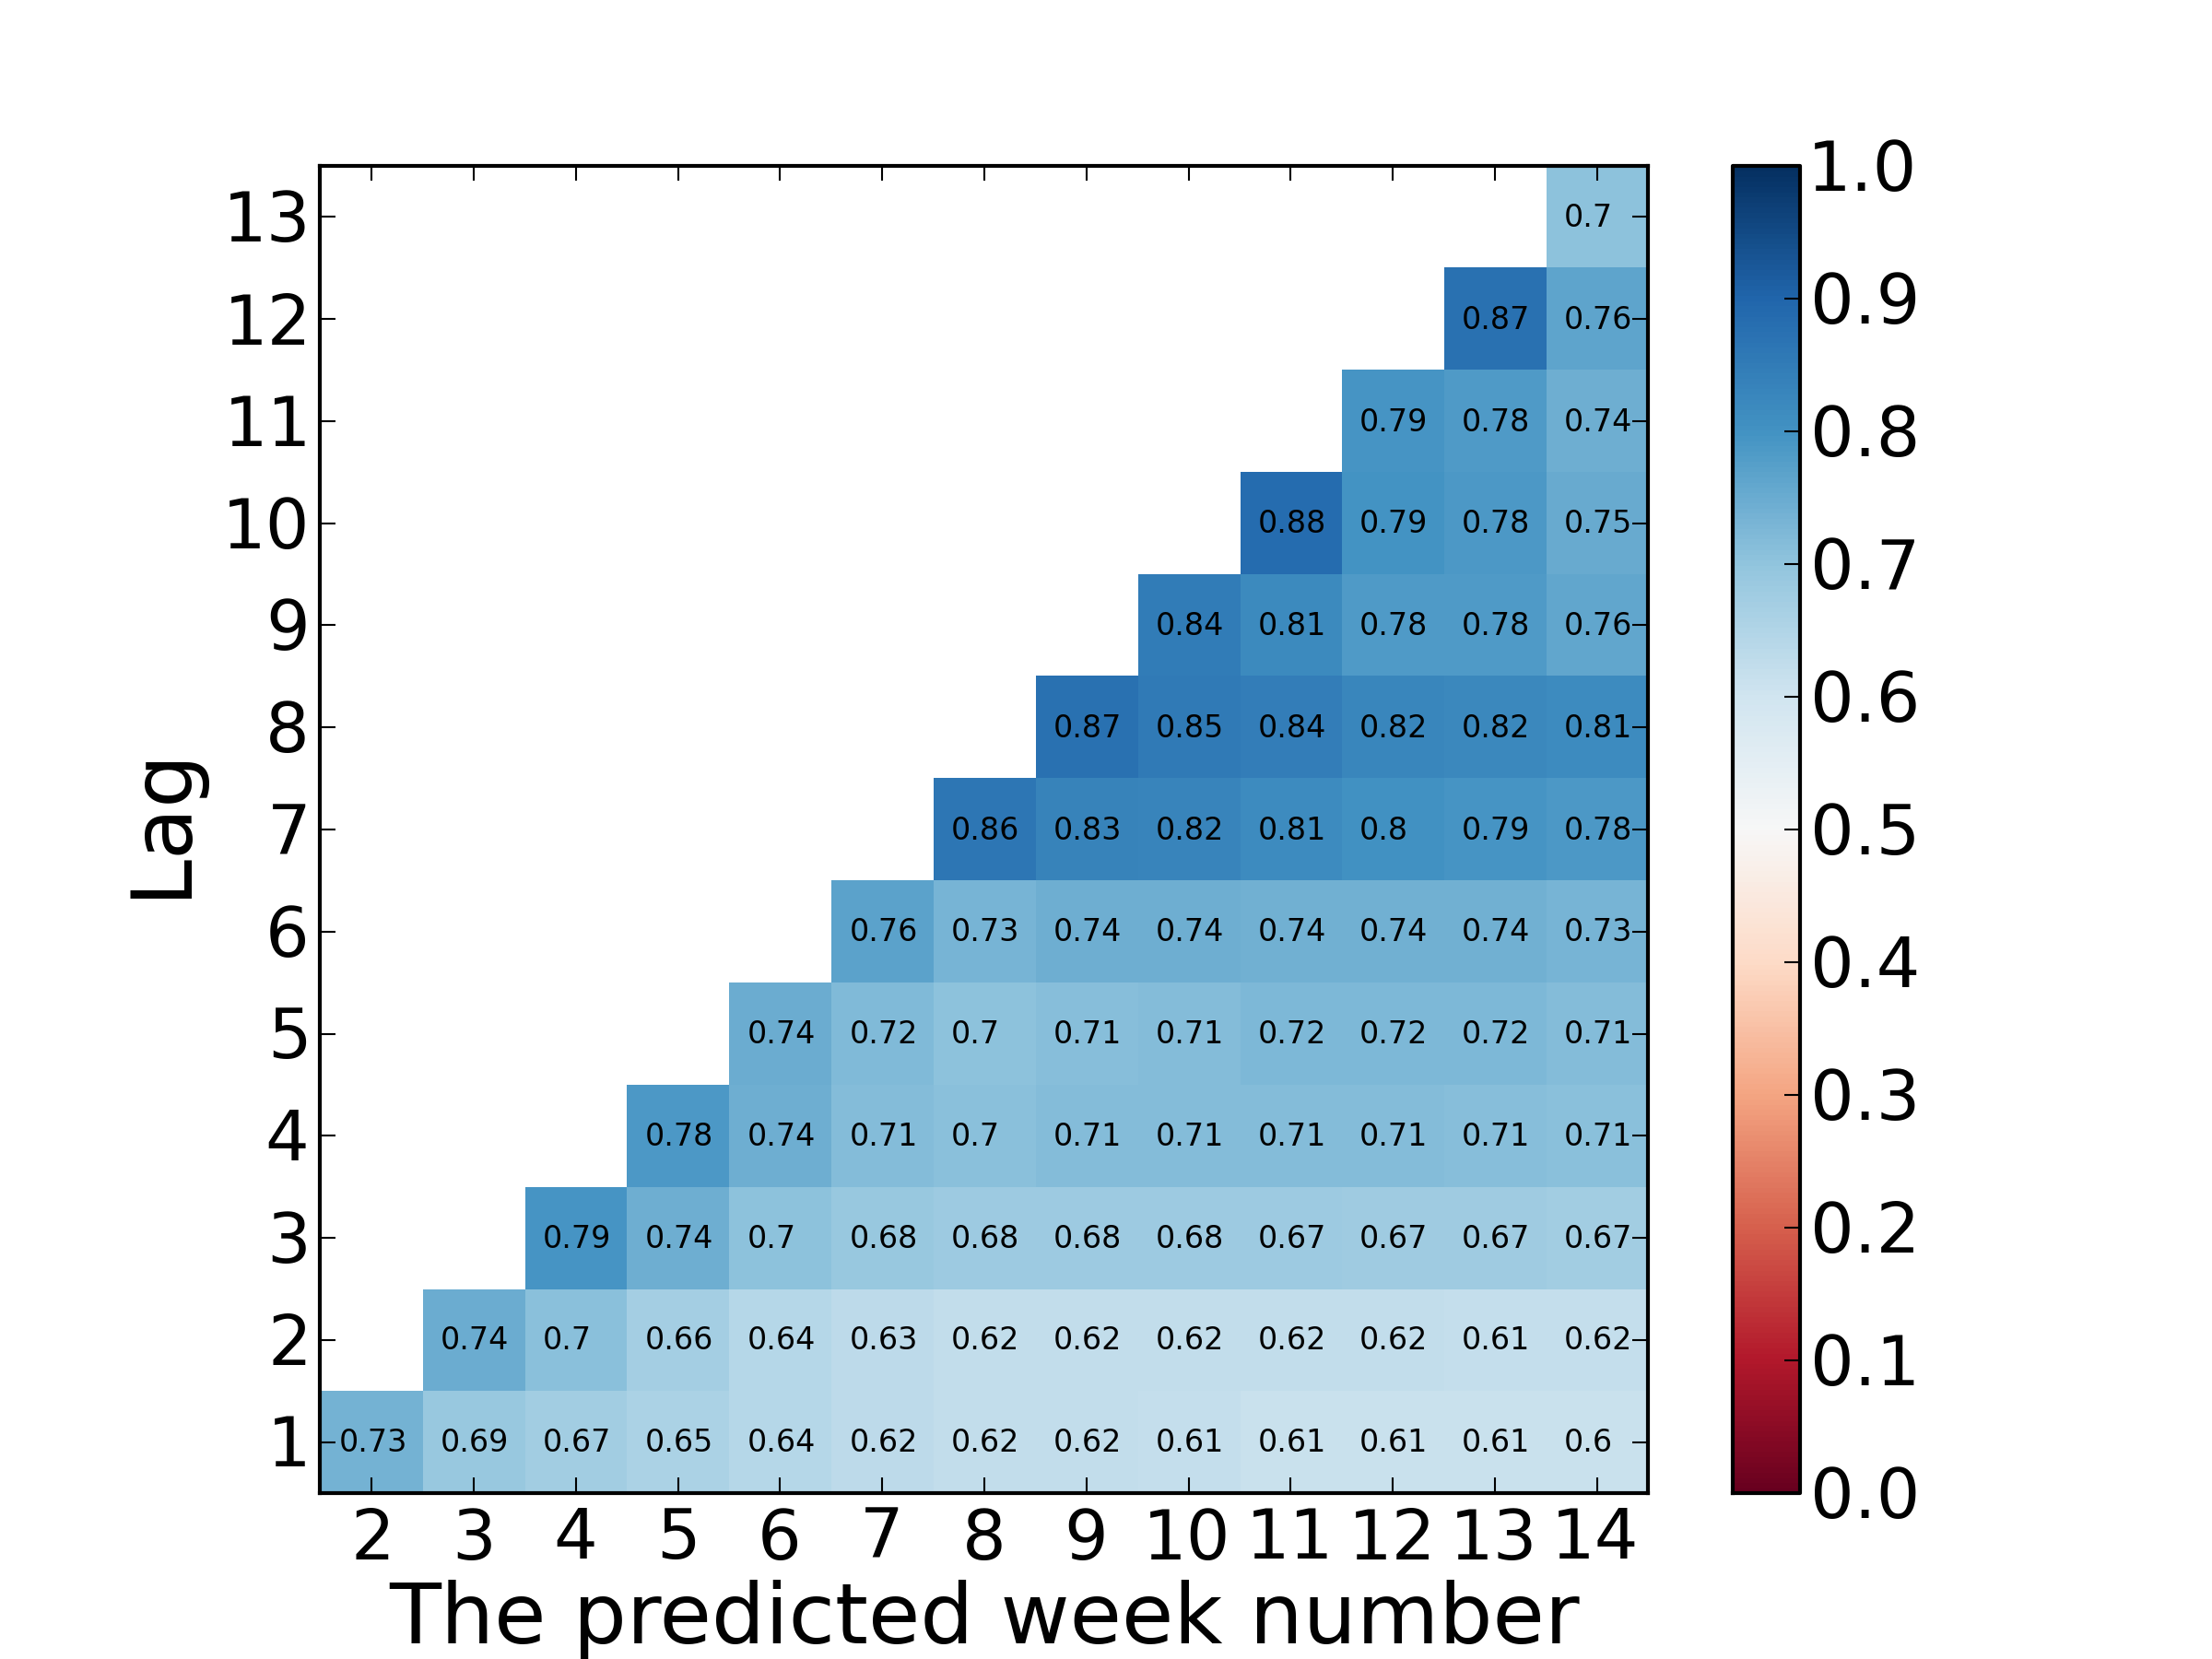
\includegraphics[width=1.0\textwidth]{figures/hmm_logreg/forum_only_pca_support_21.png}
\end{figure}

\begin{figure}[ht!]
  \caption{Heatmap of the \both cohort. PCA transformations of features used. The shown heatmap used a support of 19 for the HMM. This was the support which yielded the highest mean AUC.}\label{fig:hmm_logreg_heatmap_forum_and_wiki}
  \centering
    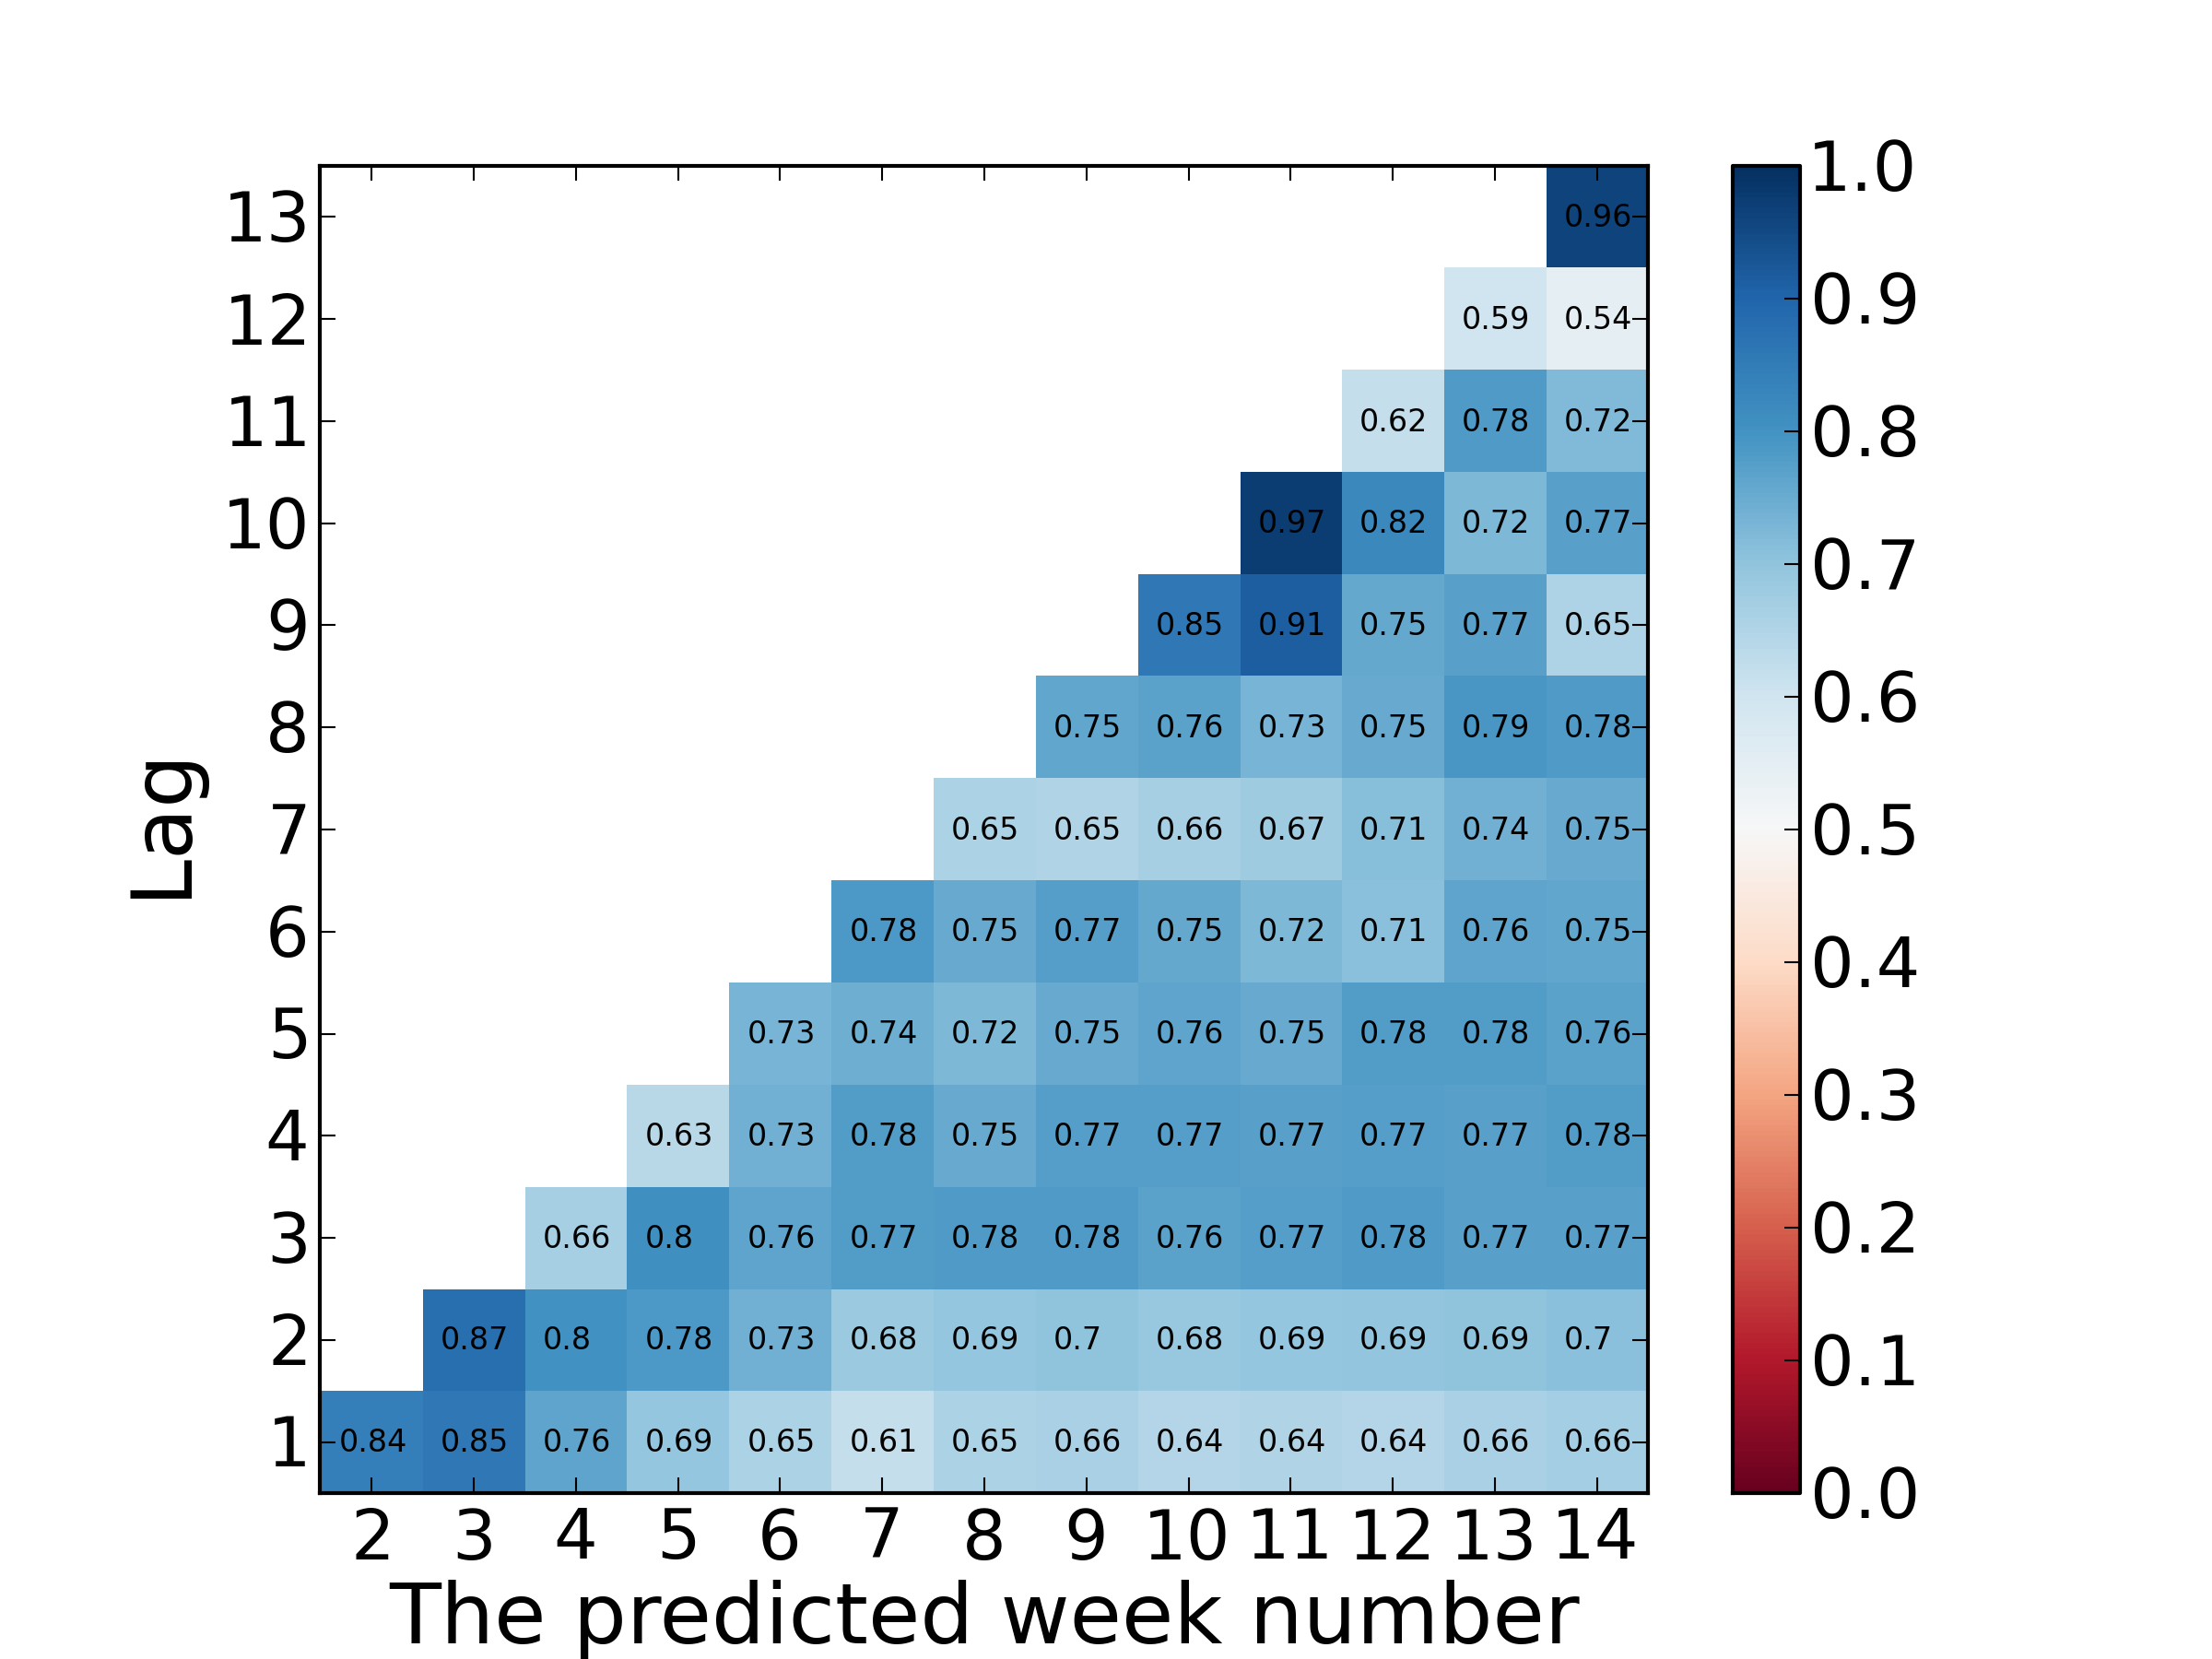
\includegraphics[width=1.0\textwidth]{figures/hmm_logreg/forum_and_wiki_pca_support_19.png}
\end{figure}

\begin{figure}[ht!]
  \caption{Heatmap of the \wiki cohort. The shown heatmap used a support of 7 for the HMM. This was the support which yielded the highest mean AUC.}\label{fig:hmm_logreg_heatmap_wiki_only}
  \centering
    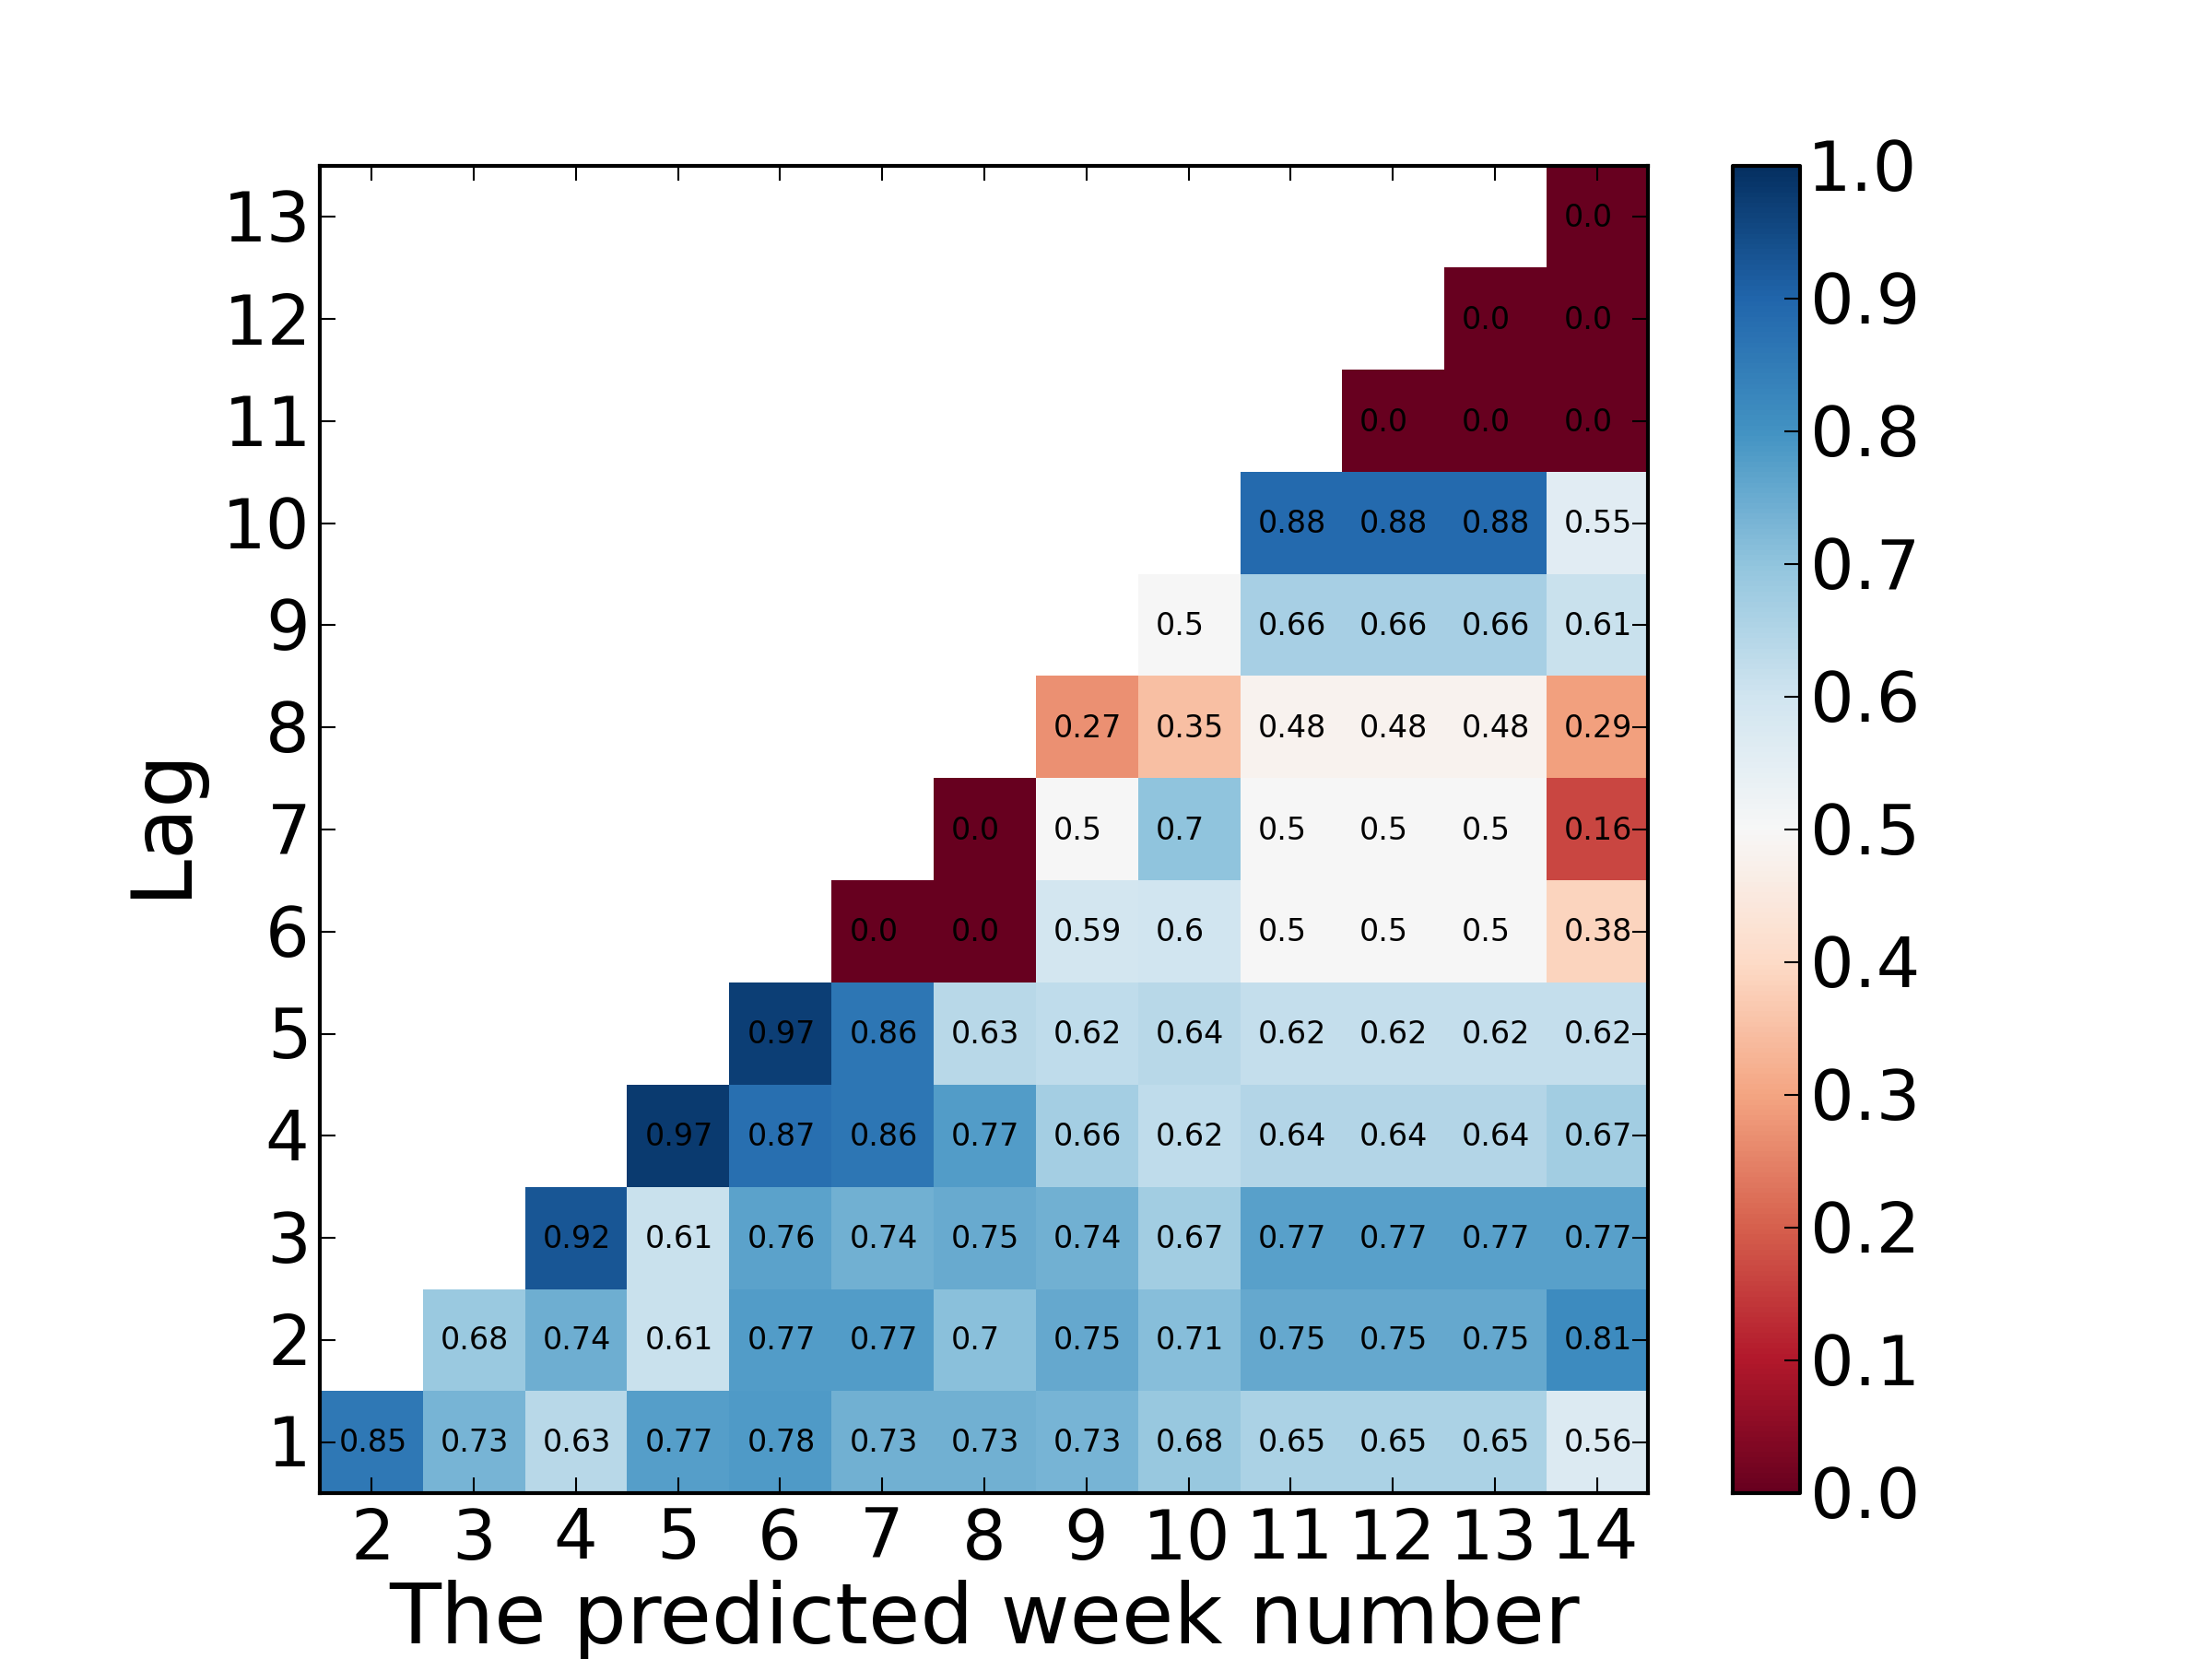
\includegraphics[width=1.0\textwidth]{figures/hmm_logreg/wiki_only_support_7.png}
\end{figure}

The HMM logistic regression models perform similarly to the logistic regression models. Their AUCs are more polarized, however, due to the constant transition matrix, as described in chapter \ref{chap:hmm}. For short leads, HMM logistic regression out-predicts logistic regression, but its performance decreases faster as the lead increases. 

\begin{figure}[ht!]
  \caption{Mean AUC as K increases for the \neither cohort. PCA transformations of features used.}\label{fig:hmm_logreg_support_over_time_no_collab_pca}
  \centering
    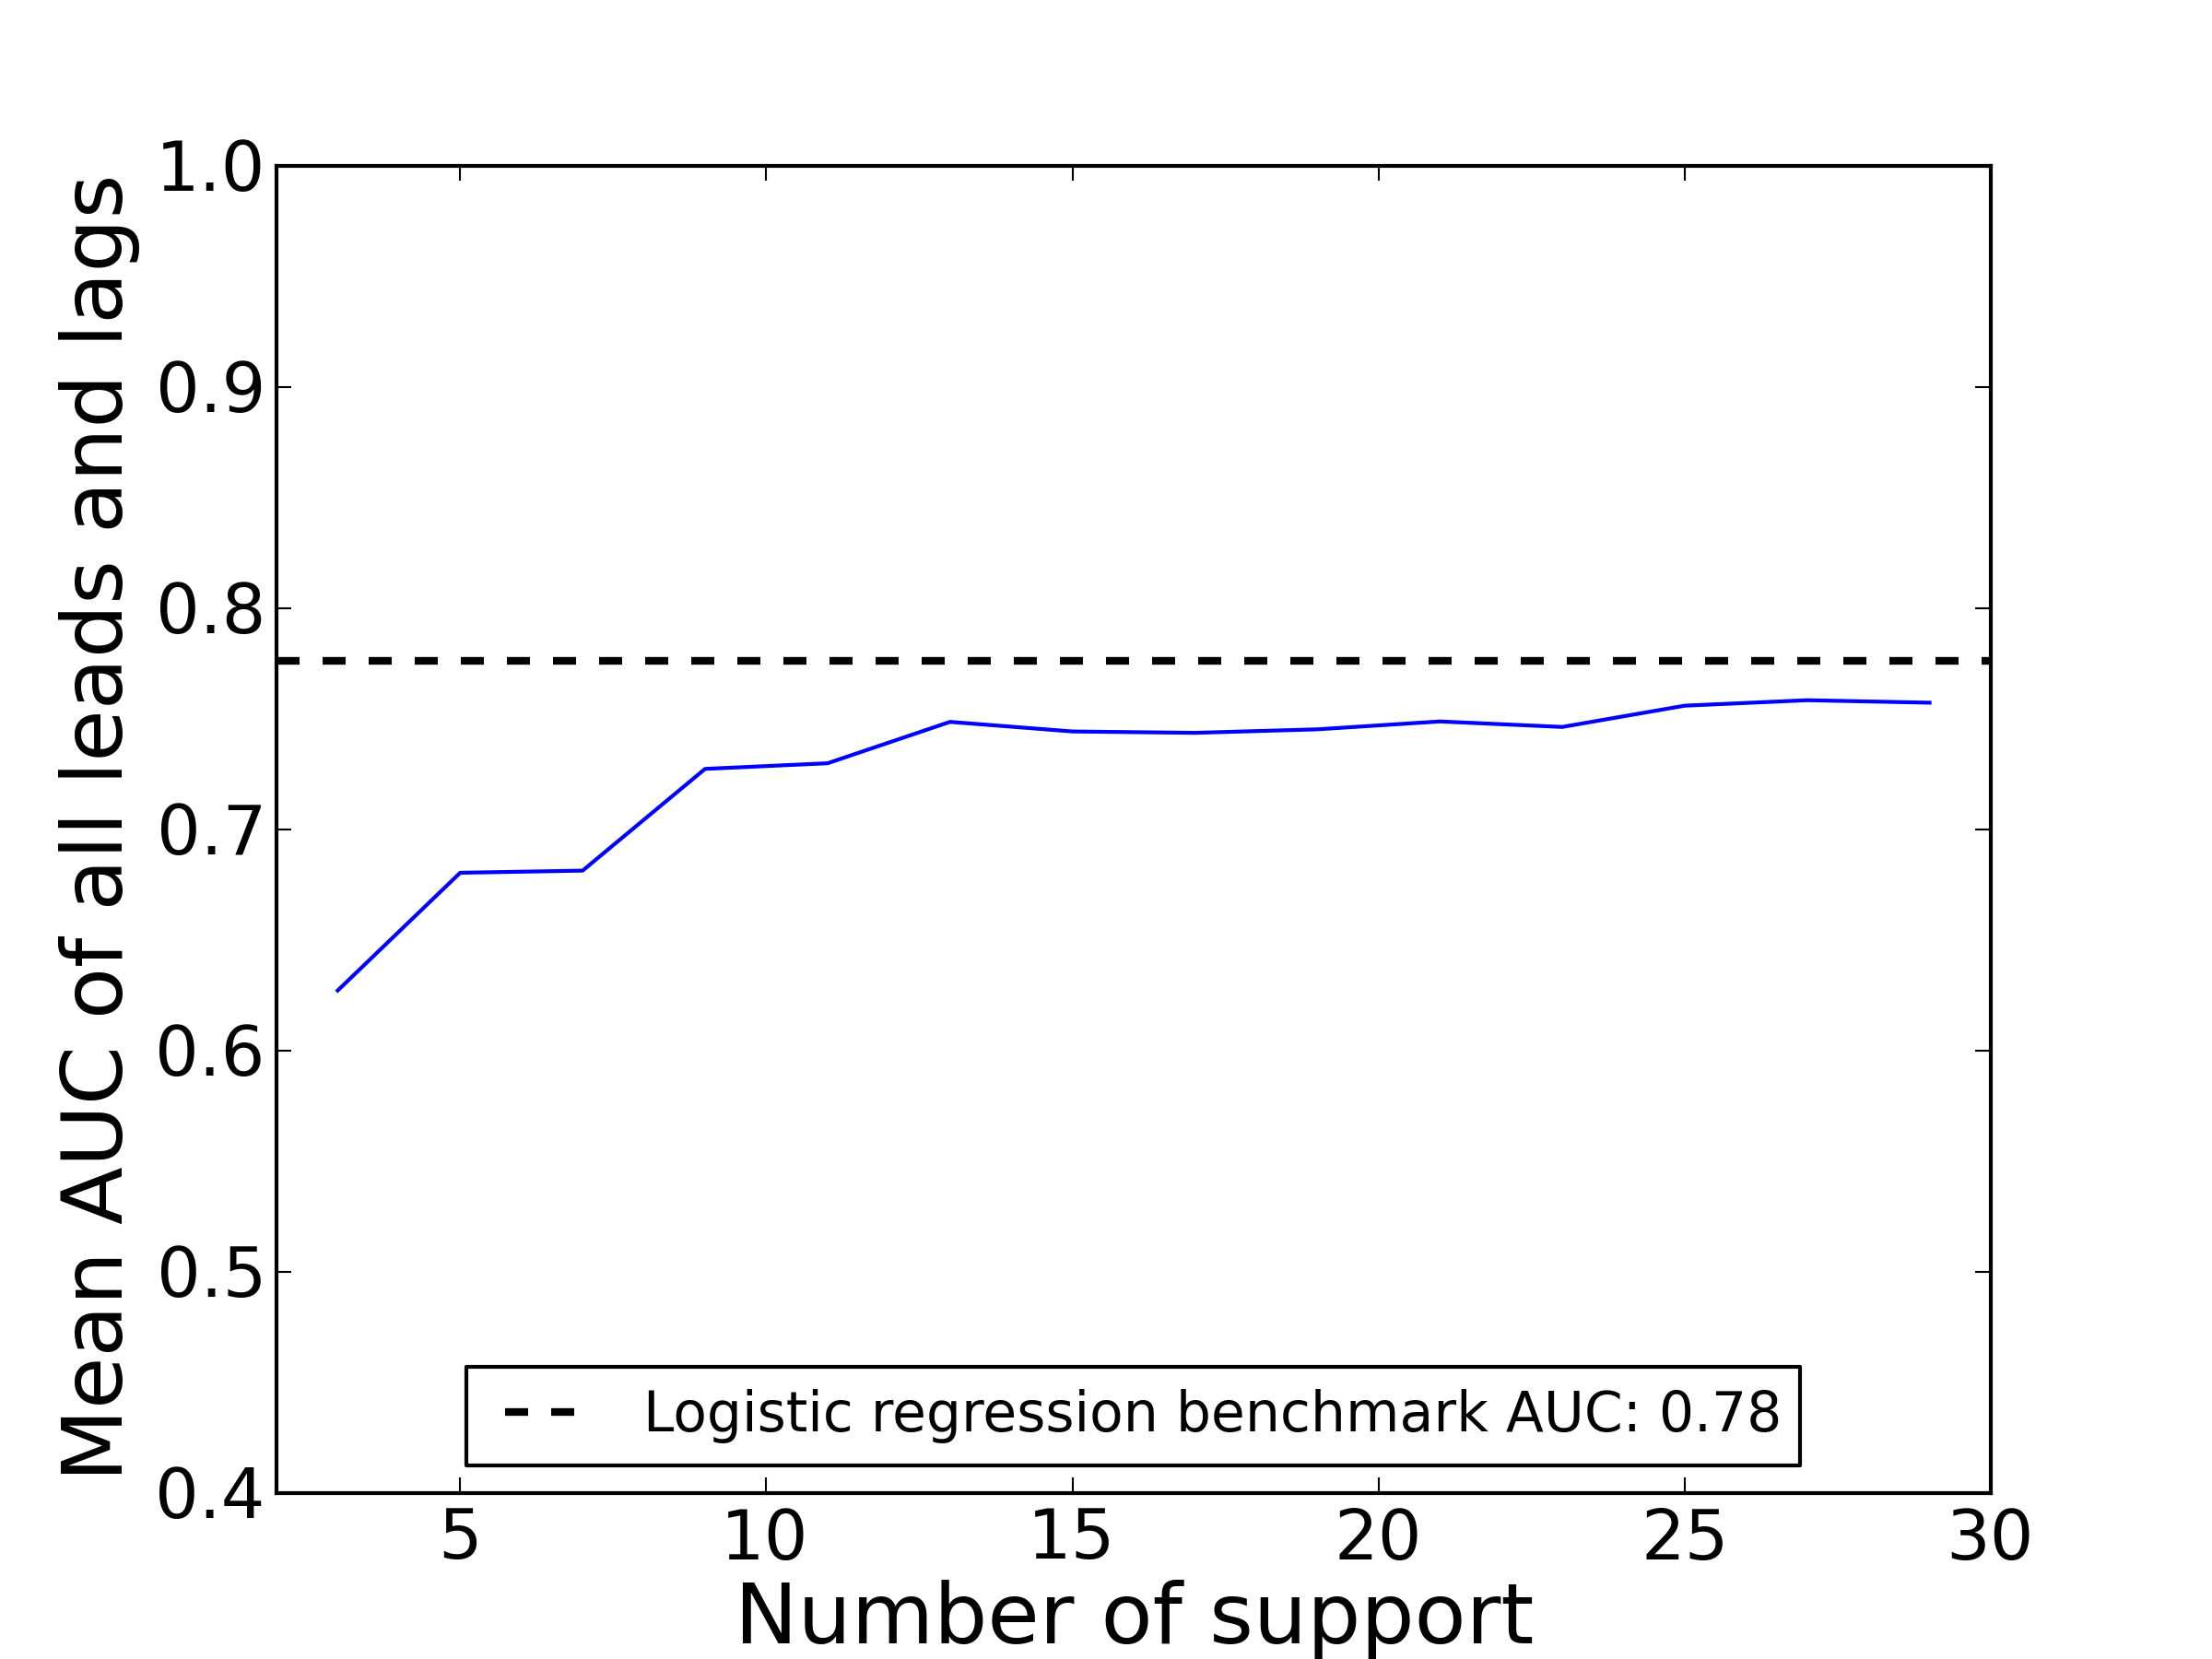
\includegraphics[width=0.8\textwidth]{figures/hmm_logreg/no_collab_pca_support_over_time.png}
\end{figure}

\begin{figure}[ht!]
  \caption{Mean AUC as K increases for the \forum cohort. PCA transformations of features used.}\label{fig:hmm_logreg_support_over_time_forum_only_pca}
  \centering
    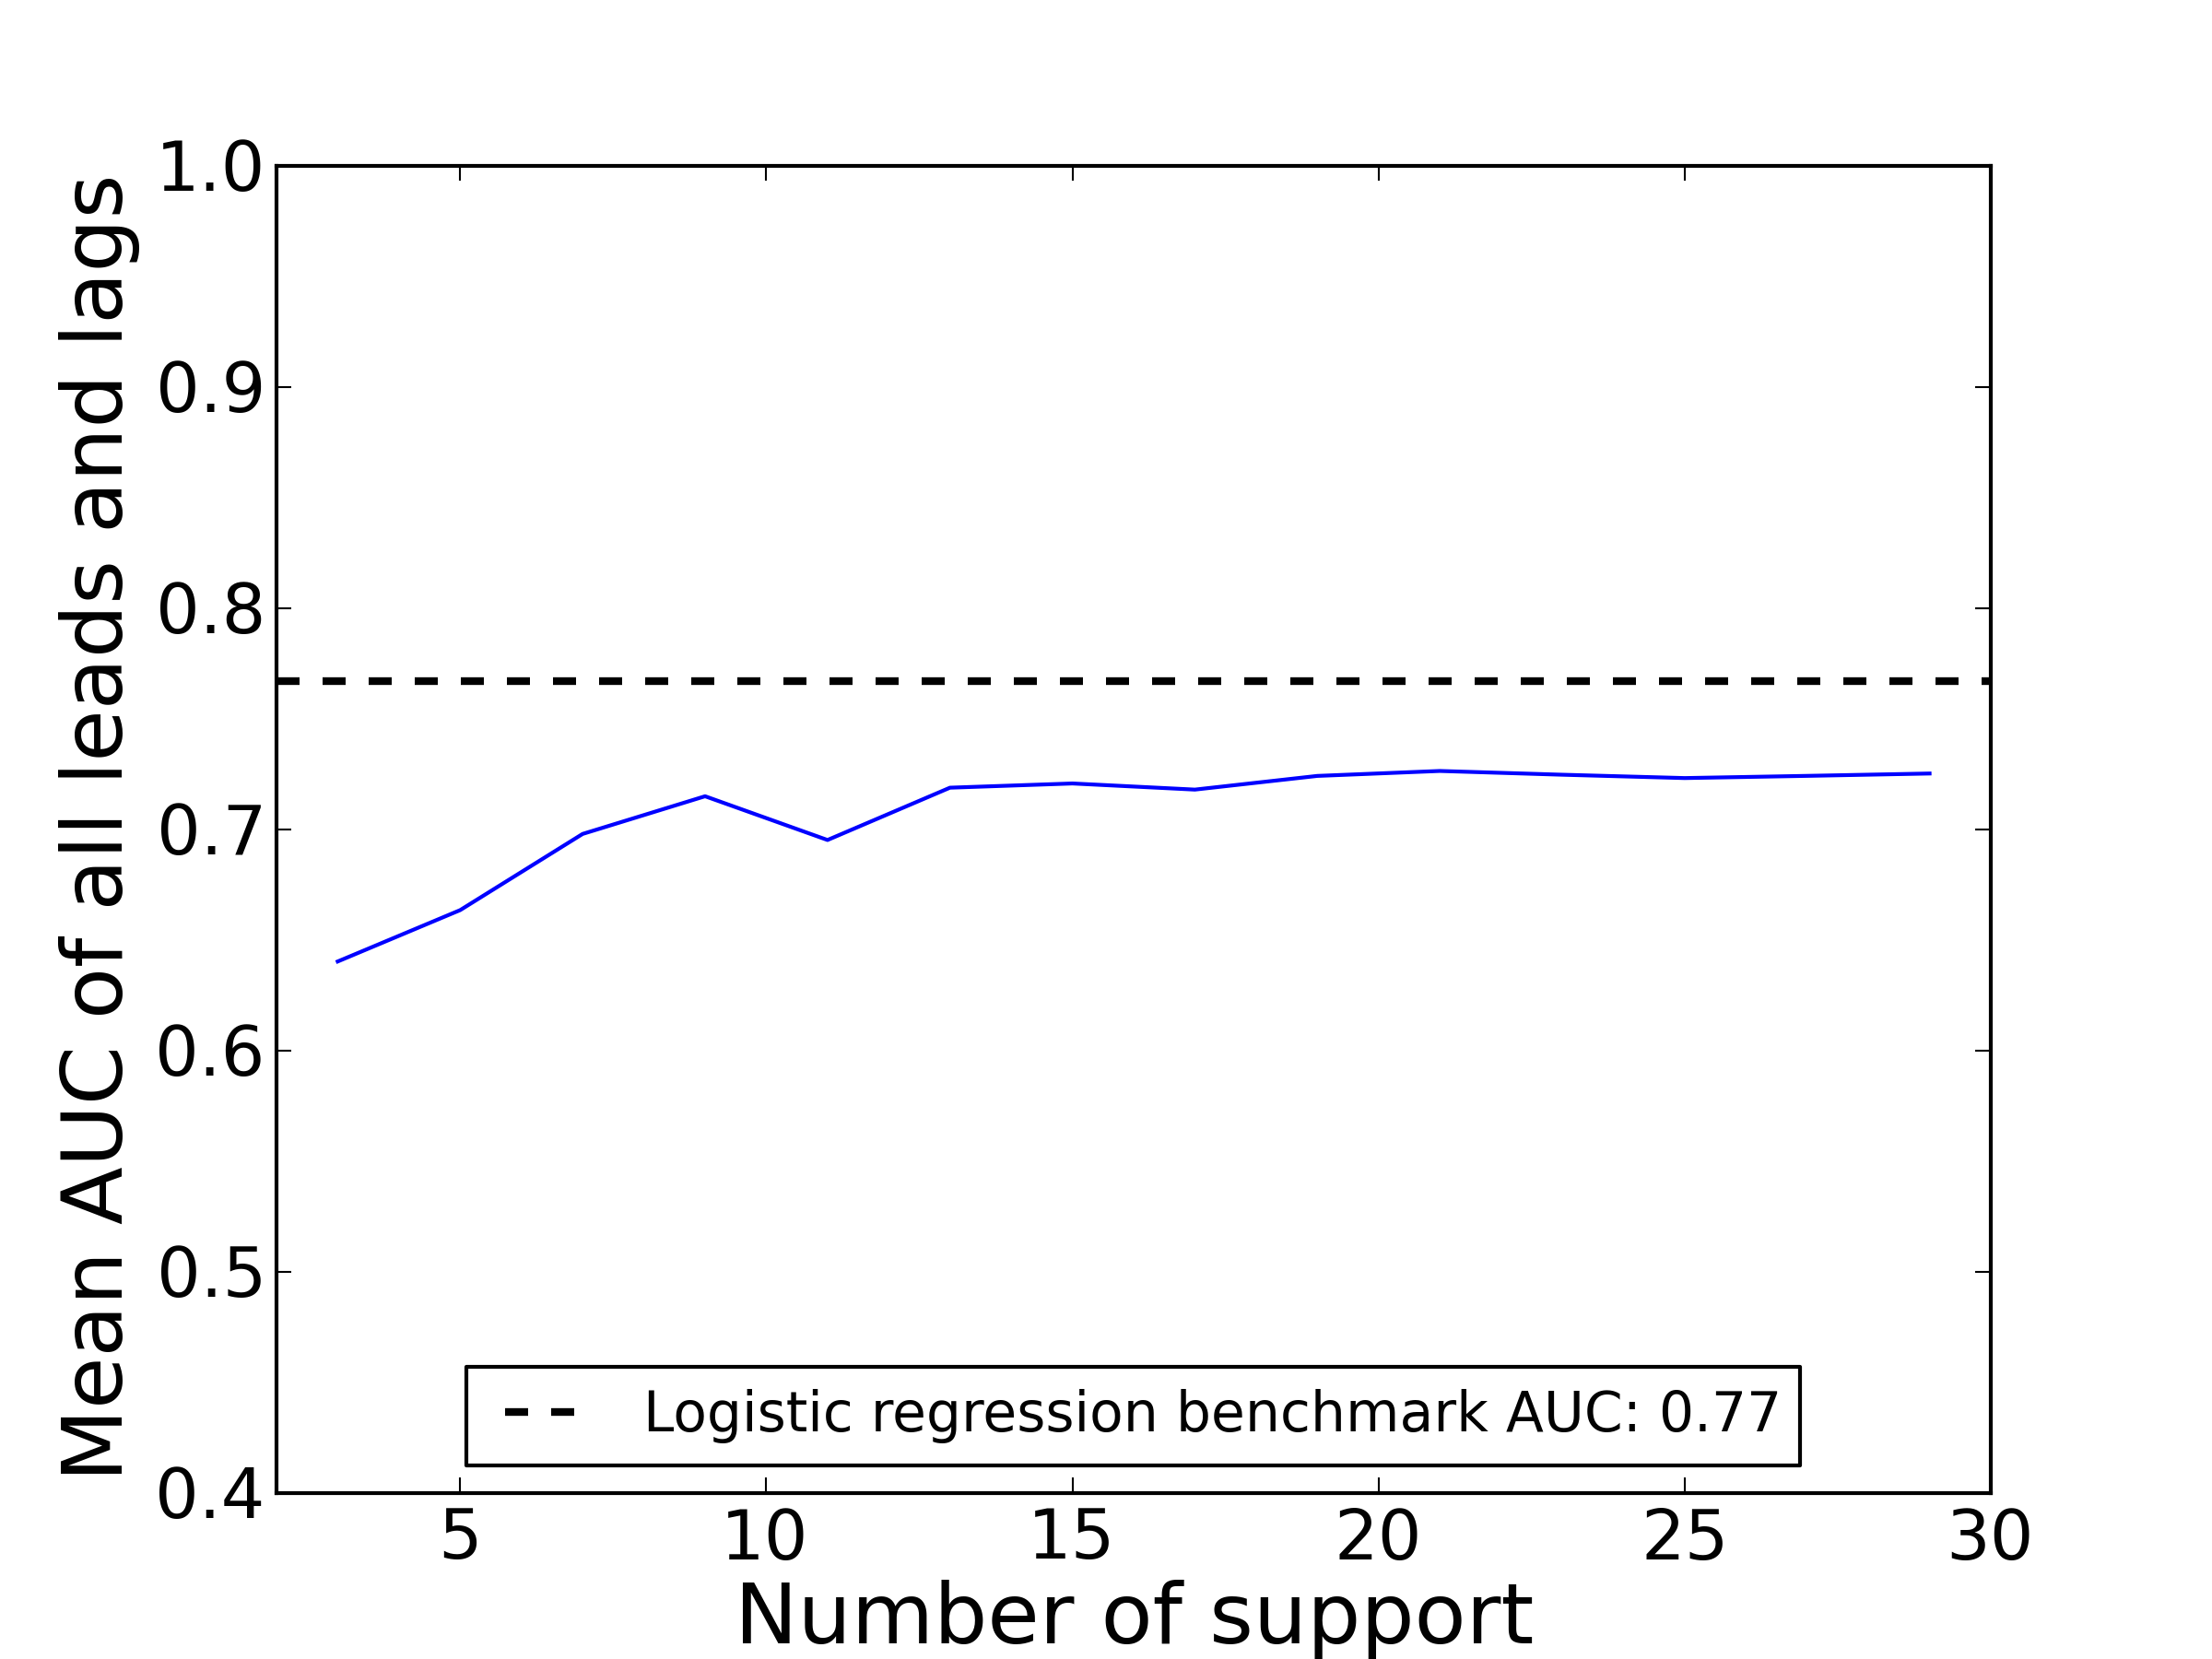
\includegraphics[width=0.8\textwidth]{figures/hmm_logreg/forum_only_pca_support_over_time.png}
\end{figure}

\begin{figure}[ht!]
  \caption{Mean AUC as K increases for the \both cohort. PCA transformations of features used.}\label{fig:hmm_logreg_support_over_time_forum_and_wiki_pca}
  \centering
    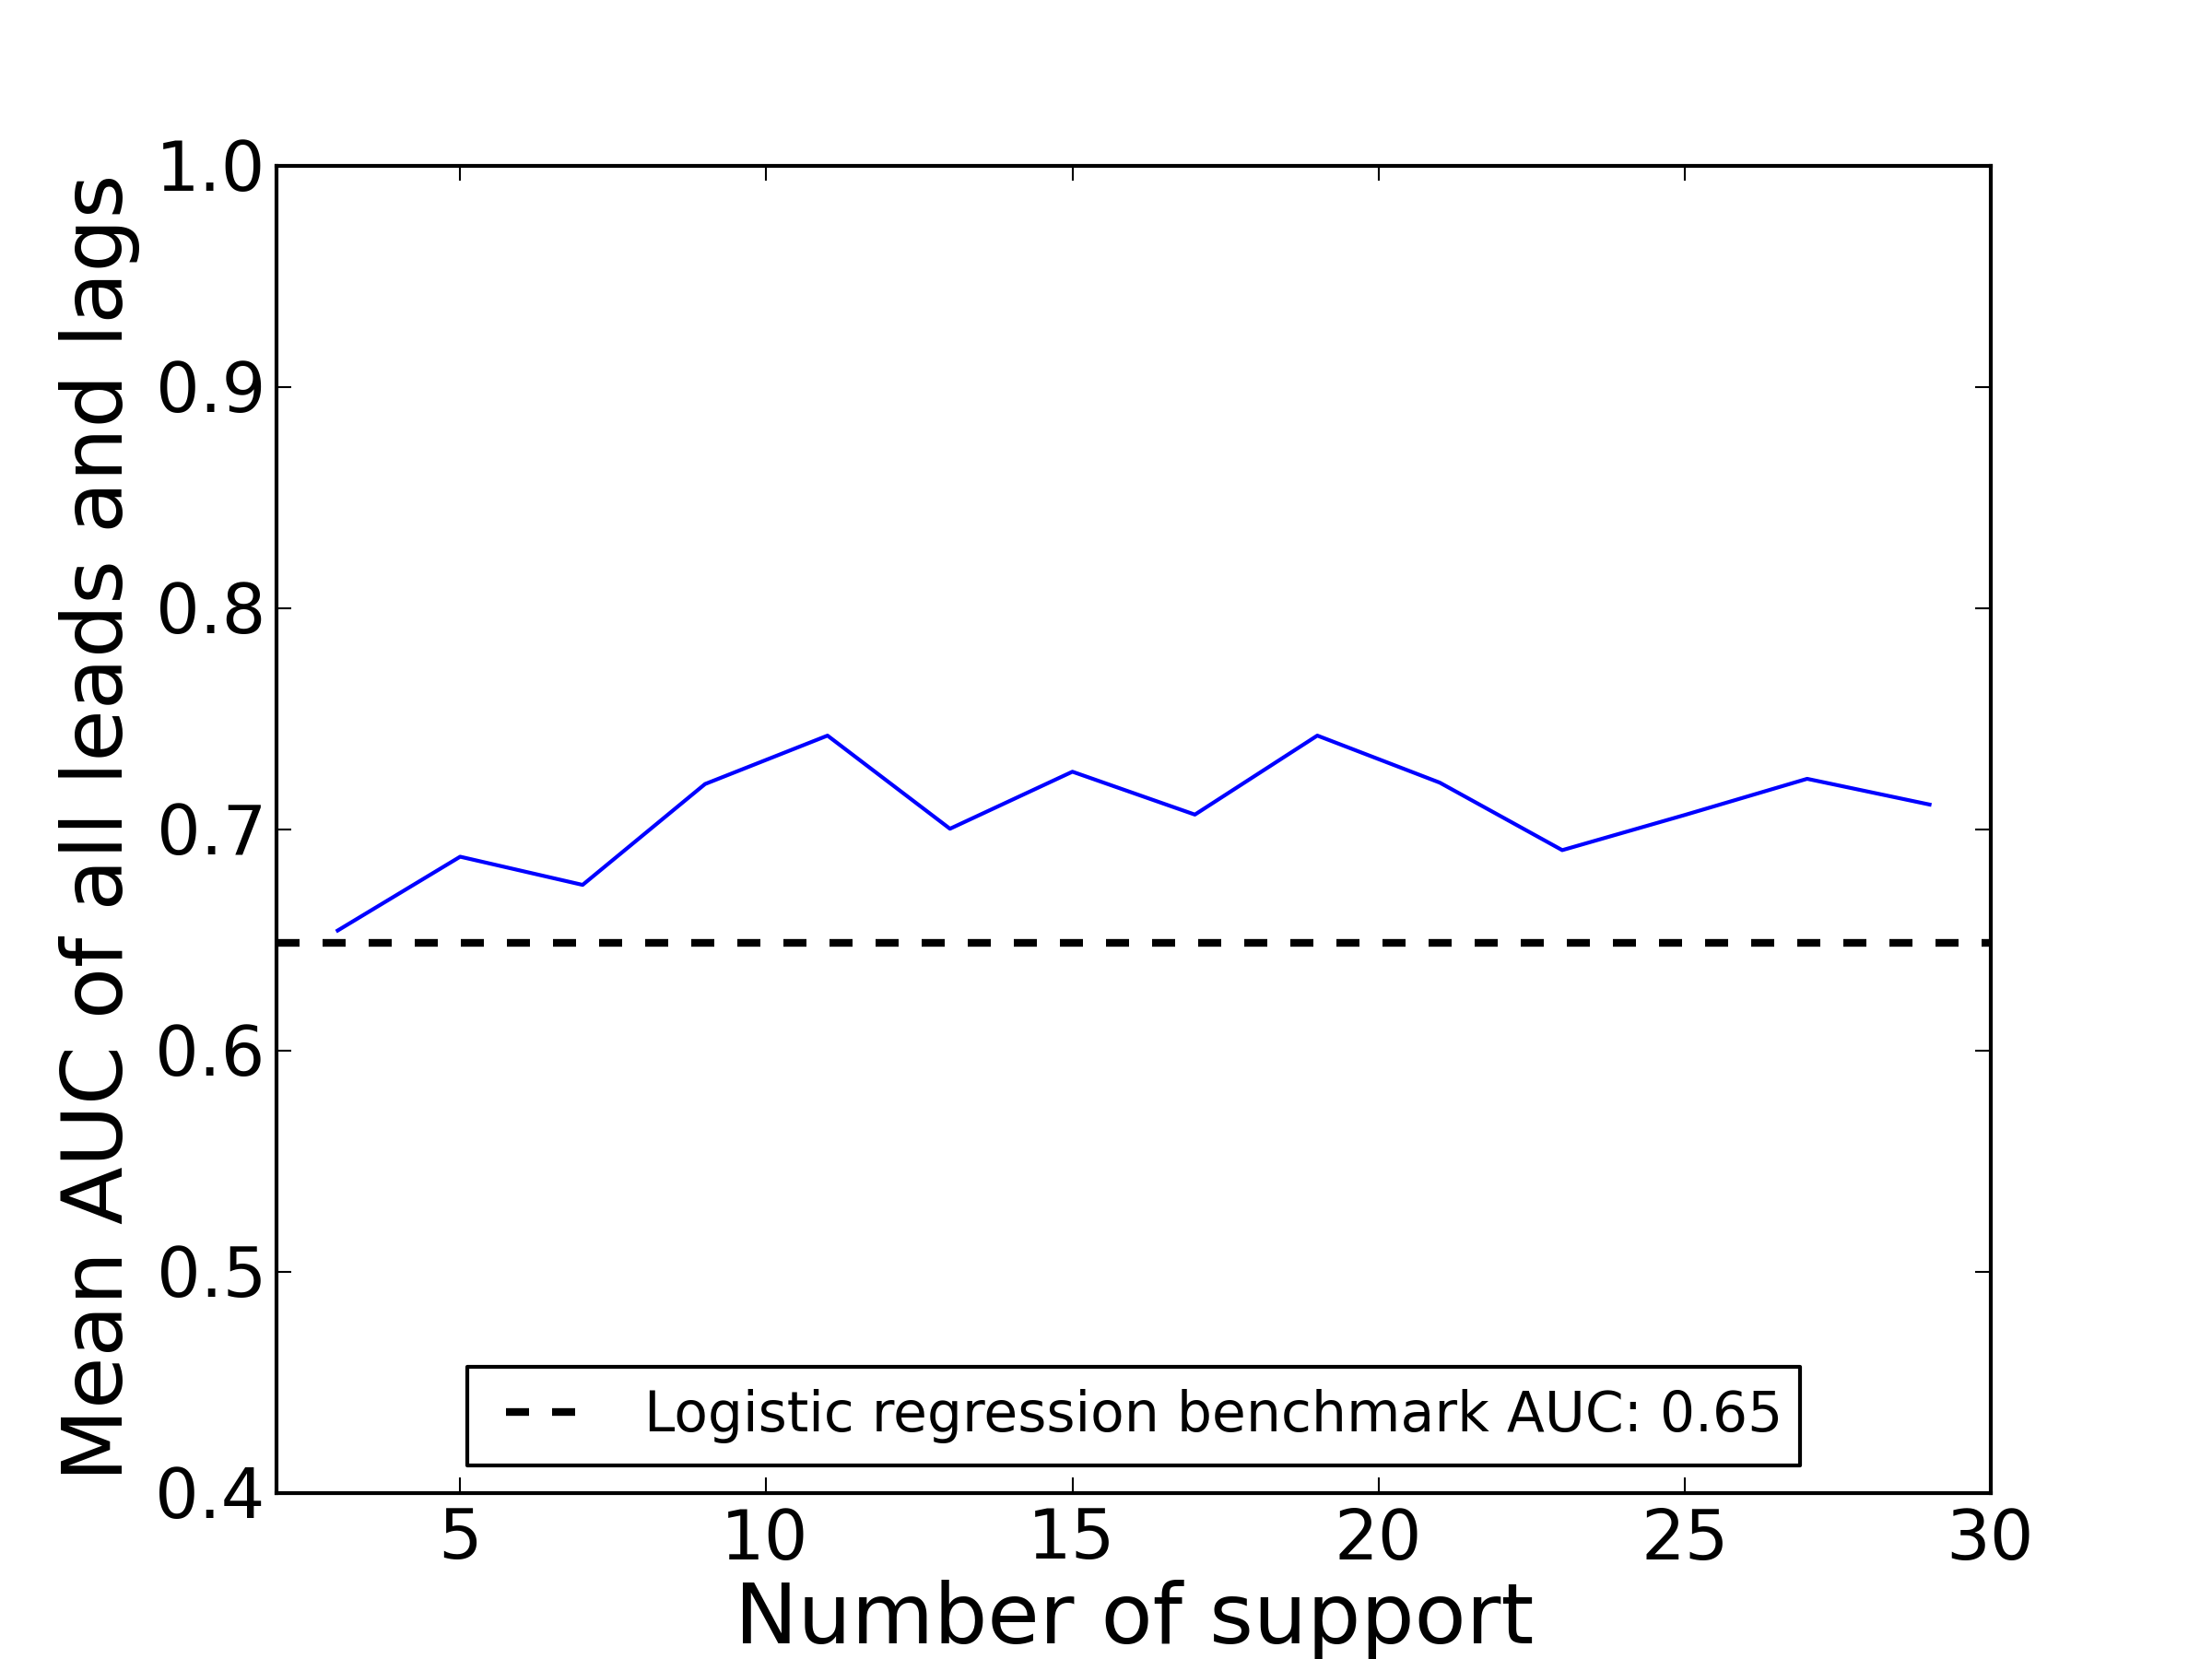
\includegraphics[width=0.8\textwidth]{figures/hmm_logreg/forum_and_wiki_pca_support_over_time.png}
\end{figure}

\begin{figure}[ht!]
  \caption{Mean AUC as K increases for the \wiki cohort.}\label{fig:hmm_logreg_support_over_time_wiki_only}
  \centering
    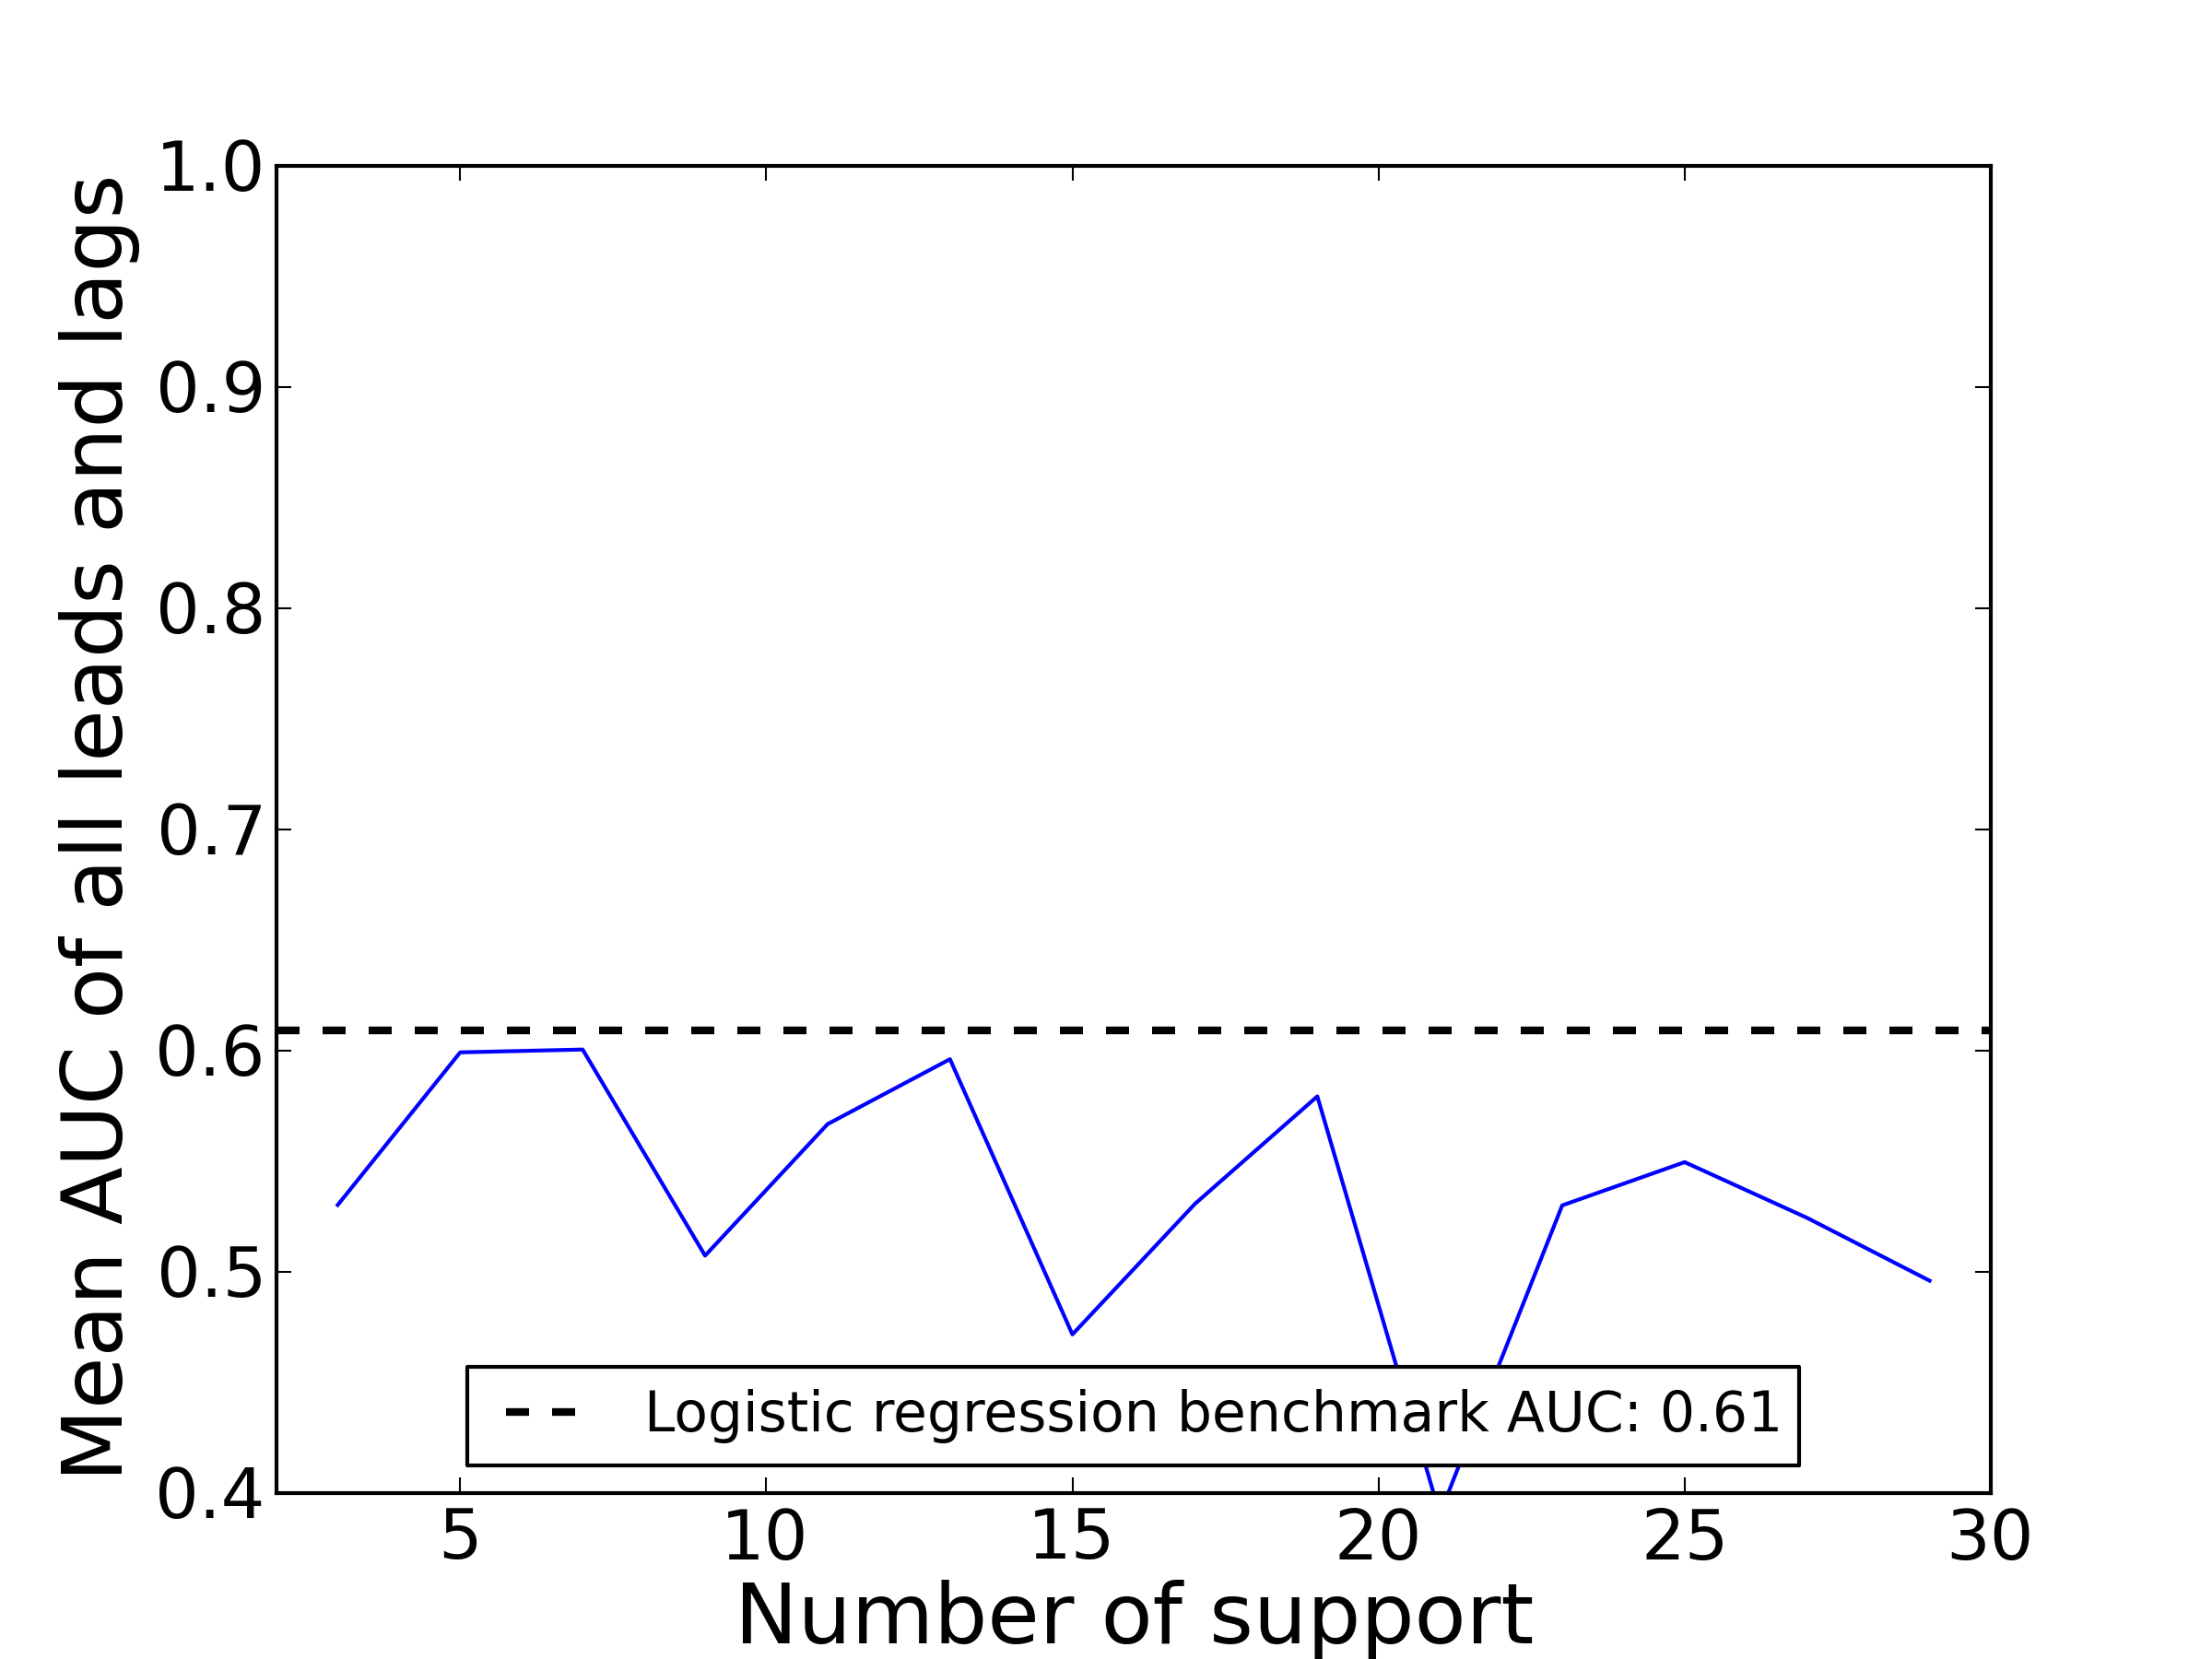
\includegraphics[width=0.8\textwidth]{figures/hmm_logreg/wiki_only_support_over_time.png}
\end{figure}

Figures \ref{fig:hmm_logreg_support_over_time_no_collab_pca} through \ref{fig:hmm_logreg_support_over_time_wiki_only} show how overall predictive accuracies of the HMM models change as K increases. The logistic regression mean AUC is also shown as a benchmark. The only cohort which outperforms logistic regression is \both, presumably because HMM model is able to train with less students. All cohorts except for \wiki converge around K of 21.